\documentclass{article}

\usepackage{microtype}
\usepackage{graphicx}
\usepackage{booktabs}
\usepackage{amsmath}
\usepackage{hyperref}

\newcommand{\theHalgorithm}{\arabic{algorithm}}

\usepackage{mlsys2025}

% arXiv preprint notice (style default says "Do not distribute")
\makeatletter
\renewcommand{\Notice@String}{Preprint.}
\makeatother

\graphicspath{{../figs/}}

% terminology macros: one word per concept
\newcommand{\x}{$\times$}

\begin{document}

\mlsystitlerunning{Fidelity Cuts vs.\ Function Cuts}

\twocolumn[
\mlsystitle{Fidelity Cuts vs.\ Function Cuts: What Compressing Speculative-Decoding Draft Heads Destroys, and How to Detect It Before Deployment}

\mlsyssetsymbol{equal}{*}

\begin{mlsysauthorlist}
% TODO(user decision): author list and affiliation pending
\mlsysauthor{Avi Fenesh}{ind}
\end{mlsysauthorlist}

\mlsysaffiliation{ind}{Independent researcher}

\mlsyscorrespondingauthor{Avi Fenesh}{}

\mlsyskeywords{speculative decoding, quantization, pruning, draft models, compression}

\vskip 0.3in

\begin{abstract}
Co-trained multi-token-prediction heads give Qwen- and DeepSeek-lineage models built-in speculative decoding at a fixed price: the head's full-vocabulary projection reads 1.34GB of weights per drafted token on a 9B model, and separate-artifact deployments hold 1 to 2GB of GPU memory. We compress the head and measure exactly what each kind of compression destroys, using the verifier itself as a per-token oracle. Every drafted token is a labeled test of whether compression changed the function. The measurements sort all compression into two families. Fidelity cuts (uniform precision reduction) cost at most 1.9 acceptance-retention points under severe domain shift, with 8-bit indistinguishable from the reference. Function cuts (channel pruning, low-rank factorization, distillation) keep 97\% of their acceptance on calibration-register text and pay 10 to 19 retention points on genuinely shifted text. The tax grows with shift distance and survives six selection schemes, including selection calibrated on the pruned head's own observed failures. The mechanism is statistical: parameters serving rare content accumulate no mass on any finite calibration sample. Three practical results follow. A zero-training recipe (trim the vocabulary to the model's own 32k hottest tokens, quantize to NVFP4, verify full-vocabulary) cuts per-token reads to 0.21GB. It delivers 1.8 to 2.7\x{} end-to-end speedup over plain decoding on Qwen3.5-9B and Qwen3.6-27B in a production CUDA engine, with outputs distribution-exact by construction. A forward-pass audit classifies any compressed draft before deployment: harm-per-disagreement separates the families (0.14 versus 0.28 to 0.54), and in-distribution disagreement ranks the off-distribution tax exactly on our hardest suite (Spearman 1.0, exact $p = 0.0002$). A measurement protocol makes sampled-decoding comparisons reproducible after we found single-prompt sampled cells swing 12 acceptance points across seeds. All negative results appear in full.
\end{abstract}
]

\section{Introduction}
\label{sec:intro}

Models in the Qwen and DeepSeek lineages ship with a co-trained multi-token-prediction head \cite{gloeckle2024better,deepseek2024v3}: one spare transformer block that drafts tokens for speculative decoding \cite{leviathan2023fast,chen2023accelerating}, trained alongside the trunk. The head reaches acceptance rates external drafters struggle to match, and it costs accordingly. Its output projection spans the full 248,320-token vocabulary, so each drafted token reads 1.34GB of weights on a 9B model. Decode is bandwidth-bound, so those reads price directly into generation speed. Deployments that load the head as a separate file also surrender 1 to 2GB of GPU memory that could hold context.

Compressing the head looks routine: the toolbox (vocabulary trimming, quantization, pruning, low-rank factorization, distillation) is mature. Choosing from it safely is the hard part. Standard practice evaluates compressed models on data resembling the calibration set, and on such data the dangerous cuts look free. We measure a pruned head that keeps 97\% of its acceptance on calibration-register text and keeps only 80\% on genuinely shifted text, a collapse the calibration-side numbers cannot reveal. Which compressions carry this hidden liability, and how a practitioner detects it before deployment, are the questions this paper answers.

The answer is a two-family taxonomy. \textbf{Fidelity cuts} reduce the numeric precision of every weight uniformly; quantization is the family. \textbf{Function cuts} remove selected structure (channels, ranks) or refit the function on selected data (distillation). Measured across seven compression arms, two models, and three evaluation corpora at increasing distance from calibration, the family alone determines shift behavior. Fidelity cuts pay at most 1.9 acceptance-retention points under severe domain shift, with 8-bit indistinguishable from the reference. Function cuts pay 10 to 19 points on the same suite, a gap of an order of magnitude, and the gap grows with shift distance. The mechanism is statistical and carries no model-specific ingredient, though our evidence spans two scales of one model lineage. The parameters serving rare content fire too rarely to accumulate mass on any finite calibration sample, so every selection statistic misses exactly the function that shift will demand. We test six selection schemes, including one calibrated on the pruned head's own observed failures. All six fail identically.

Draft heads are the right place to establish this, twice over. Verification makes draft errors free: a wrong draft costs latency and leaves the output untouched, so the head tolerates aggressive fidelity loss. Verification also labels every drafted token against ground truth, which makes compression damage countable per token at a scale no task benchmark matches.

This paper contributes:

\begin{enumerate}
\item \textbf{A zero-training compression recipe.} Trim the head's vocabulary to the model's own 32k hottest tokens, quantize the remainder to NVFP4, keep full-vocabulary verification. The head's per-token reads drop from 1.34GB to 0.21GB and verification keeps the output distribution exact by construction.

\item \textbf{The fidelity/function taxonomy with the evidence that makes it actionable.} A 2$\times$2 design separates dimensionality from calibration-dependence: data-free SVD pays more than calibrated SVD, so dimensionality itself is the liability. The six-scheme study shows the function-cut tax survives every zero-training selection statistic.

\item \textbf{A pre-deployment audit that needs no shifted data.} Running the compressed head beside its reference on in-distribution documents yields two numbers: disagreement rate and harm per disagreement. Harm classifies the family (0.14 for fidelity cuts versus 0.28 to 0.54 for function cuts). Disagreement ranks the off-distribution tax exactly (Spearman 1.0, exact $p = 0.0002$, on the domain-shift suite).
\end{enumerate}

On Qwen3.5-9B and Qwen3.6-27B in a production CUDA engine, the recipe delivers 1.8\x{} and 2.2\x{} on a short-prompt suite, and 2.0\x{} and 2.7\x{} on a long-context suite, from 212MB and 259MB draft artifacts. Every cell aggregates 80 or 20 prompts and three sampling seeds. The fastest 27B long-context cell reaches 128.6 tokens per second against 47.7 for plain decoding. An independently built third configuration reproduces the recipe's pattern. The negative results that shaped the taxonomy, six failed selection schemes, two falsified mechanisms, and one retracted headline, appear in full, together with the measurement protocol that makes sampled-decoding comparisons reproducible.

\section{Setting: Draft Heads, and Verification as an Oracle}
\label{sec:setting}

\subsection{Co-trained draft heads}
\label{sec:heads}

Speculative decoding accelerates autoregressive generation by drafting $K$ candidate tokens cheaply and verifying them with one batched pass of the target model \cite{leviathan2023fast,chen2023accelerating}. Classical pipelines draft with a separate small model, which must exist, fit in memory, and match the target's distribution. Co-trained multi-token-prediction heads \cite{gloeckle2024better,deepseek2024v3} remove those requirements: the model ships with one extra transformer block, trained jointly with the trunk, that predicts ahead from the trunk's hidden state. The head inherits the trunk's distribution by construction and reaches acceptance rates external drafters struggle to match.

The built-in convenience carries a fixed cost with two parts (Figure~\ref{fig:anatomy}). The output projection spans the full vocabulary: 248,320 rows at Qwen3.5 scale, 1.08GB of 8-bit weights read per drafted token. The block itself adds 0.26GB. Decode-time inference is bandwidth-bound, so at $K{=}4$ the head's 5.3GB of reads per round competes directly with the target's own weights for the same memory bus. Deployments that load the head as a separate artifact pay in capacity as well: 1 to 2GB of a consumer GPU's memory that could hold context.

\begin{figure}[t]
\centering
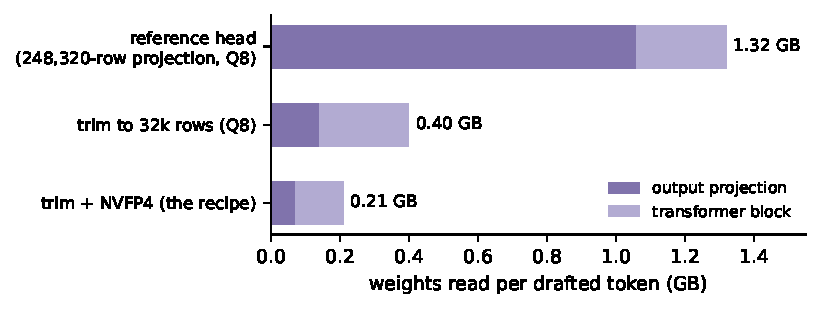
\includegraphics[width=\columnwidth]{f0_cost_anatomy.pdf}
\caption{Weights read per drafted token on Qwen3.5-9B. The full-vocabulary output projection dominates the reference head's cost; the recipe (\S\ref{sec:recipe}) cuts total reads 6.3\x.}
\label{fig:anatomy}
\end{figure}

\subsection{The verifier as a measurement instrument}
\label{sec:oracle}

Two properties make draft heads the right laboratory for studying compression. First, drafting is error-tolerant by construction. The target verifies every drafted token; a wrong draft costs one round of wasted speculation and never changes the output. Compression errors that would corrupt a base model only slow a draft head down. Second, verification labels every drafted token against ground truth. Each position yields an exact, binary, task-grounded measurement of whether compression changed the function's behavior there, at a scale of millions of labeled positions per GPU-hour. Classifier benchmarks measure compression damage through task metrics with their own noise; the verifier measures it directly. We use the first property to justify aggressive compression and the second to measure precisely what each kind of compression destroys.

\section{The Cut Taxonomy and the Recipe}
\label{sec:taxonomy}

\subsection{Where the bytes go}
\label{sec:bytes}

The co-trained head is one transformer block plus an output projection over the full vocabulary. On Qwen3.5-9B the projection is $248{,}320 \times 4096$ (1.08GB at 8-bit) and the block is roughly 243M parameters (0.26GB), so a single drafted token reads 1.34GB. Speculative decoding drafts $K$ tokens per round, so at $K{=}4$ the head reads 5.3GB per verify pass. Every compression method attacks this budget somewhere: the projection's rows, the block's precision, the block's channels or rank, or the whole function. We group the methods by what they remove (Figure~\ref{fig:taxonomy}). \textbf{Fidelity cuts} lower the numeric precision of every weight and leave the function's structure intact. \textbf{Function cuts} remove structure: channels, ranks, or the function itself in favor of a retrained substitute.

\begin{figure}[t]
\centering
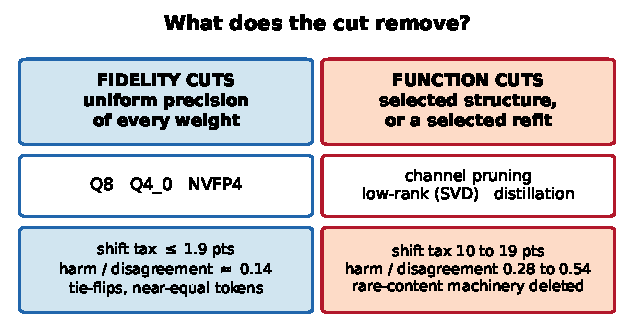
\includegraphics[width=\columnwidth]{f6_taxonomy.pdf}
\caption{The two-family taxonomy with its measured signatures. Family membership alone predicts behavior under distribution shift (\S\ref{sec:robust}) and the audit's harm rate (\S\ref{sec:audit}).}
\label{fig:taxonomy}
\end{figure}

\subsection{Trim: remove outputs, keep computation}
\label{sec:trim}

Trim ranks vocabulary rows by frequency over text the model itself generated and keeps the top 32,768 plus every special token, following the load-time trimming direction of FR-Spec \cite{zhao2025frspec}. A draft-to-target index map converts the trimmed head's argmax back to full-vocabulary token ids, and verification runs against the full vocabulary. Trim's damage model is therefore explicit. A draft whose correct continuation falls outside the hot set proposes a wrong token, verification rejects it, and the round loses speed, never correctness. The tax equals the coverage gap and nothing else: within the hot vocabulary the trimmed head computes the identical function. Coverage is 95 to 99\% of generated tokens on our suites, and unlike a function cut's damage, the gap is measurable on any traffic sample before deployment. Trim deletes no computation. Every channel, head, and rank still executes; only output rows the draft would rarely propose disappear. It is also the reason trim creates no further pruning headroom. We measured the hot-logit energy of every FFN channel: each channel spreads its output over hot and cold rows in proportion to their count. Deleting cold rows orphans no channel.

\subsection{Fidelity cuts: uniform precision loss}
\label{sec:fidelity}

Quantizing the head's matrices to 8-bit or 4-bit blocks perturbs every weight by a small rounding error. The perturbation is uniform by construction: the rounding selects no weight, so it singles out no sub-function for damage. The draft setting makes this nearly free twice over. A draft error costs one round of latency and never correctness, because the target verifies every token; and the head's job, ranking likely continuations, survives logit noise that would matter in a lossless setting. Our 4-bit format is NVFP4 (16-element blocks, e2m1 values, fp8 sub-scales), the project's deployment standard; Q4\_0 behaves the same within noise. Section~\ref{sec:robust} quantifies the family's worst case at 1.9 retention points under severe domain shift, with 8-bit indistinguishable from the reference.

\subsection{Function cuts: selection is the liability}
\label{sec:function}

Channel pruning and low-rank factorization remove specific structure, chosen either by a statistic over calibration data or, for data-free SVD, by the weight matrix's own spectrum. Distillation replaces the head with a smaller one trained on chosen data. All three tie the surviving function to a finite sample: the calibration set, the spectrum's large directions, or the training distribution. Content that the sample under-represents loses its machinery, and \S\ref{sec:robust} shows the loss arrives exactly there, at 10 to 19 retention points under domain shift. The six-scheme study in \S\ref{sec:selection} shows the liability follows from selection itself: statistics computed on finite samples cannot see rare-firing function, whatever the statistic.

Distillation deserves one scoping sentence. A distilled replacement reaches 91 to 98\% of the teacher's chain acceptance on its training register at 13\% of the compute. It is the only option when a model ships no co-trained head, or when a quantized base breaks the head it has. When a strong co-trained head exists, the trained substitute never beat the trimmed original in our aggregate cells, and it inherits the function-cut robustness profile.

\subsection{The recipe}
\label{sec:recipe}

The safe moves compose: trim the projection (structural, coverage-capped, shift-proof in \S\ref{sec:robust}) and quantize what remains (uniform, 1.9 points worst case). One command exports the artifact from a HuggingFace checkpoint: rank the vocabulary on the model's own output, gather the hot rows, quantize head and block to NVFP4, and emit a standalone draft file with the index map. The 9B artifact is 212MB against the natural head's 1.34GB of per-token reads; the 27B artifact is 259MB. No training step exists anywhere in the pipeline, so the recipe runs on the deployment machine in minutes.

\section{Evaluation}
\label{sec:eval}

\subsection{Setup}
\label{sec:setup}

We evaluate on Qwen3.5-9B and Qwen3.6-27B, two dense hybrid models that ship co-trained MTP heads, running in bw24, a production CUDA engine, on a single RTX PRO 6000 (96GB). Two prompt suites cover the serving range. The short suite is MT-Bench: 80 prompts across eight categories, 256 generated tokens each. The long suite is 20 prompts of 1.9k to 5.9k tokens (documents with analysis instructions, long code files with review instructions), 512 generated tokens each. Each cell reports acceptance (accepted drafts over drafted tokens at $K{=}4$) and end-to-end tokens per second against the same-suite plain-decode baseline, for greedy decoding and for temperature 0.7 with three sampling seeds.

The aggregate protocol is itself a finding. A single-prompt sampled cell swings by 12 acceptance points across four seeds, and twenty seeds on one long prompt span 57 points (standard deviation 13): the sampler wanders into a different trajectory, and acceptance reflects whatever content appears. The spread is format-independent (Q8 and NVFP4 heads swing alike, sd 13.2 versus 14.0), so no quantization choice buys it back. Toggling an attention-kernel variant moves the trajectory the same way. Suite-level aggregation with three seeds brings the acceptance spread under 1.5 points on the 80-prompt suite, whose aggregate speedups then move at most 0.04\x{} across seeds; we interpret speedup gaps at or under 0.04\x{} as ties. The 20-prompt long suite still moves several tenths under sampling, so we rank arms on greedy cells and quote its sampled cells as three-seed means. Every number below is an aggregate; we report single-prompt cells nowhere. One earlier headline of ours (a 2.68\x{} sampled cell) failed this protocol; we retracted it in the lab record.

\textbf{Arms.} The reference is the unmodified head. Trim replaces the 248,320-row output projection with the 32,768 rows ranked hottest on the model's own generated text, plus an index map into the full vocabulary. Verification stays full-vocabulary, so greedy output stays identical and sampled output stays distribution-exact by the standard speculative guarantee \cite{leviathan2023fast,chen2023accelerating}. Trim-Q8 and trim-NVFP4 quantize all head matrices to 8-bit and 4-bit blocks on top of the trim. The robustness study (\S\ref{sec:robust}) adds channel pruning at two budgets, low-rank factorization at a byte-matched rank in data-free and calibrated variants, and the distilled replacement head.

\subsection{The recipe matches or beats every arm end to end}
\label{sec:e2e}

Table~\ref{tab:grid} reports the full grid, and Figure~\ref{fig:headline} plots the greedy cells. On the 9B short suite, trim-NVFP4 reaches 262.8 tok/s (1.82\x{} over plain decode) against 256.5 (1.78\x) for trim-Q8 and 219.1 (1.52\x) for the unmodified head. On the 9B long suite the ordering tightens: trim-Q8 292.3 (2.04\x), trim-NVFP4 282.5 (1.98\x), unmodified 245.8 (1.72\x). At 27B the 4-bit arm leads outright. It reaches 103.3 tok/s (2.15\x) on the short suite, tying Q8 to the decimal at half the head bytes. On the long suite it reaches 127.5 tok/s (2.67\x), ahead of Q8's 123.6 and the unmodified head's 115.3. Sampled cells track greedy with a 0.1 to 0.2\x{} penalty across all arms.

\begin{table}[t]
\caption{End-to-end results, greedy aggregate cells: acceptance at $K{=}4$ and speedup over the same-suite plain-decode baseline. Trim-mixed pairs the NVFP4 projection with a Q4\_0 block at the same 212MB. Sampled cells (temperature 0.7, three seeds) track greedy with a 0.1 to 0.2\x{} penalty.}
\label{tab:grid}
\vskip 0.1in
\centering
\small
\begin{tabular}{llcc}
\toprule
Suite & Arm & Acceptance & Speedup \\
\midrule
9B short  & reference   & 50.1\% & 1.52\x \\
          & trim-Q8     & 47.0\% & 1.78\x \\
          & trim-NVFP4  & 45.6\% & \textbf{1.82\x} \\
          & trim-mixed  & 45.1\% & 1.81\x \\
\midrule
9B long   & reference   & 61.6\% & 1.72\x \\
          & trim-Q8     & 60.0\% & 2.04\x \\
          & trim-NVFP4  & 54.7\% & 1.98\x \\
          & trim-mixed  & 58.3\% & \textbf{2.09\x} \\
\midrule
27B short & reference   & 53.2\% & 2.02\x \\
          & trim-Q8     & 50.4\% & \textbf{2.15\x} \\
          & trim-NVFP4  & 48.6\% & \textbf{2.15\x} \\
          & trim-mixed  & 44.7\% & 2.04\x \\
\midrule
27B long  & reference   & 69.7\% & 2.42\x \\
          & trim-Q8     & 69.5\% & 2.59\x \\
          & trim-NVFP4  & 67.5\% & 2.67\x \\
          & trim-mixed  & 68.2\% & \textbf{2.70\x} \\
\bottomrule
\end{tabular}
\end{table}

\begin{figure}[t]
\centering
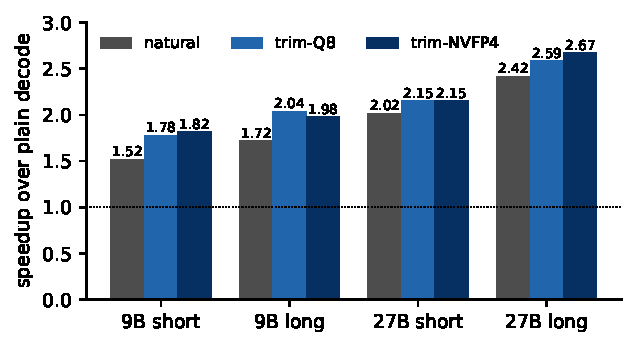
\includegraphics[width=\columnwidth]{f1_headline.pdf}
\caption{Speedup over plain decode across both models and suites (greedy aggregate cells). Trim-NVFP4 is fastest or tied-fastest everywhere, and every arm's gain grows with target scale (\S\ref{sec:scale}).}
\label{fig:headline}
\end{figure}

Acceptance explains the shape. Trimming costs 0 to 3 acceptance points (at 27B long, 0.2 points) because hot-vocabulary coverage on generated text is 95 to 99\%. Four-bit quantization costs another 1.4 to 5.3 points. The bandwidth saving buys those points back everywhere except one cell (9B long greedy, where Q8's higher acceptance wins by 3\%). A third configuration built independently in the engine's own lane, with a different vocabulary ranking and a q4\_K block, reproduced the pattern and beat its own prior champion on both speed and acceptance.

The 4-bit cost sits in the block, and a mixed export recovers it. Pairing the NVFP4 projection with a Q4\_0 block, at a byte-identical 212MB, keeps 58.3\% acceptance on the 9B long suite against all-NVFP4's 54.7\%, and its 2.09\x{} takes that suite outright. At 27B the pattern repeats on the long suite, where the mixed export reaches 128.6 tok/s (2.70\x), the fastest cell we measure, while all-NVFP4 keeps the short-suite lead (2.15\x{} against 2.04\x). The projection tolerates any 4-bit format for free; the block's codec sets the remaining acceptance, and the deployment picks it per suite.

\textbf{Takeaway.} A trimmed, fully 4-bit head is a 212MB artifact and the fastest or tied-fastest arm in every aggregate cell, with zero training and unchanged outputs; within the family, the block codec picks the winner.

\subsection{Robustness separates the families by an order of magnitude}
\label{sec:robust}

We measure each compressed arm's acceptance retention (arm accuracy over reference accuracy on identical states, conditioned on hot-vocabulary targets) on three corpora at increasing distance from the calibration distribution. The conditioning separates the two budgets a deployment pays: retention measures what compression did to the retained function, and trim's coverage gap is a separate budget, directly measurable on any traffic sample (\S\ref{sec:limitations} quantifies it per register). The first is held-out generated documents (in-distribution). The second is fresh generations on unseen topics (same register). The third is a genuine domain-shift suite of German, Chinese, Hebrew, and Russian Wikipedia, PubMed abstracts, and C4 web text, on which the reference head's own accuracy drops from 0.88 to 0.36.

The tax divides the arms into two families. Figure~\ref{fig:tax} traces all seven arms across the three corpora, and Table~\ref{tab:retention} gives the values. Fidelity cuts stay within noise of free: Q8 retains 99.8 to 99.9\% everywhere, and the 4-bit arms retain 97.5 to 99.4\%, a worst-case tax of 1.9 points with a confidence interval that includes zero. Function cuts pay 10 to 19 points on the domain-shift suite: 16.8 for pruning at 25\% keep, 10.2 at 50\% keep, 16.8 to 18.7 for the low-rank arms. The family gap of 14.5 retention points is significant at the permutation-test floor for seven arms (label permutation over the family assignment; $p = 0.029$ is the smallest value seven arms admit), and every function-cut tax individually excludes zero at 95\% confidence. The same ordering appears on the same-register corpus at one tenth the magnitude: same-register evaluation understates the effect that deployment will see.

\begin{figure}[t]
\centering
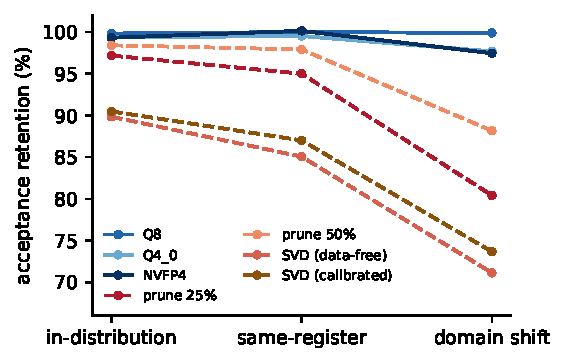
\includegraphics[width=\columnwidth]{f2_tax_by_family.pdf}
\caption{Acceptance retention versus shift distance for all seven arms. Solid blue: fidelity cuts. Dashed red: function cuts. Family membership alone determines the trajectory, and the separation grows with shift distance.}
\label{fig:tax}
\end{figure}

\begin{table}[t]
\caption{Acceptance retention (\%) by corpus, and the shift tax (in-distribution retention minus domain-shift retention, in points). Positions per corpus: 2,500 in-distribution, 2,500 same-register, 2,500 domain-shift.}
\label{tab:retention}
\vskip 0.1in
\centering
\small
\begin{tabular}{lcccc}
\toprule
Arm & In-dist & Same-reg & Dom-shift & Tax \\
\midrule
Q8          & 99.8 & 100.0 & 99.9 & $-0.1$ \\
Q4\_0       & 99.4 & 99.5  & 97.7 & 1.7 \\
NVFP4       & 99.3 & 100.1 & 97.5 & 1.9 \\
\midrule
prune 25\%  & 97.2 & 95.0  & 80.4 & 16.8 \\
prune 50\%  & 98.4 & 97.9  & 88.2 & 10.2 \\
SVD (data-free)  & 89.9 & 85.1 & 71.1 & 18.7 \\
SVD (calibrated) & 90.5 & 87.0 & 73.7 & 16.8 \\
\bottomrule
\end{tabular}
\end{table}

The taxonomy also survives quantization of the base model itself. A cross on the 9B model pairs each head arm with a bf16 base and an NVFP4-quantized base, since deployed bases are rarely full-precision. Head-compression costs stay base-independent: the 4-bit head costs 4.5 acceptance points against the bf16 base and 6.0 against the quantized base, and each compressed head's absolute acceptance moves under one point across bases. Fidelity cuts to head and base compound in speed rather than in damage. The quantized base decodes 32\% faster on its own, and adding the trim-NVFP4 head reaches 292.7 tokens per second, 2.03\x{} over bf16 plain decode.

The full grid replicates on Qwen3.6-27B. On the same domain-shift suite, re-extracted through the 27B trunk, fidelity taxes stay at or under 1.5 points and function taxes run 7.6 to 12.7 points. The family gap survives the model change.

Two internal comparisons localize the cause. Data-free SVD pays a larger tax than calibration-weighted SVD at equal rank, so dimensionality itself drives the damage, independent of calibration data. And pruning's tax concentrates in rare-token bins while the low-rank tax spreads across all bins (Figure~\ref{fig:bins}), yet both pay: selective cuts choose different function to delete, and shift surfaces the deletion either way.

\begin{figure}[t]
\centering
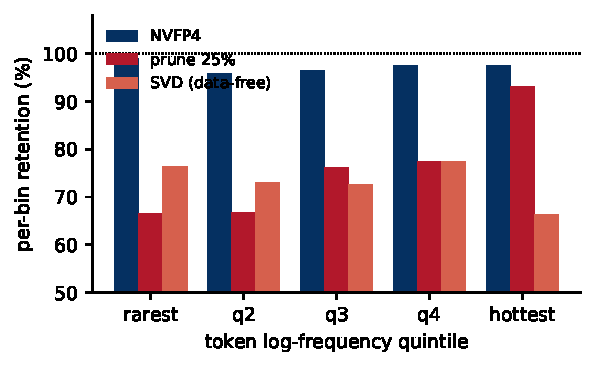
\includegraphics[width=\columnwidth]{f3_per_bin.pdf}
\caption{Per-bin retention under domain shift by token log-frequency quintile. Pruning's damage concentrates in rare bins (66\% at the rarest, 93\% at the hottest); the low-rank arm damages every bin; NVFP4 stays near 97\% throughout.}
\label{fig:bins}
\end{figure}

\textbf{Takeaway.} Under genuine distribution shift, function cuts cost an order of magnitude more acceptance than fidelity cuts, the gap widens with shift distance, and the effect is invisible to in-distribution evaluation.

\subsection{Speedups grow with target scale}
\label{sec:scale}

Every arm gains more at 27B than at 9B: the unmodified head goes from 1.52\x/1.72\x{} (short/long) to 2.02\x/2.42\x, and trim-NVFP4 from 1.82\x/1.98\x{} to 2.15\x/2.67\x. The draft's cost shrinks relative to the target's verify pass as the target grows, so each accepted token buys more. Draft compression compounds with this trend: the cheaper the round, the higher the optimal speculation depth the deployment can afford. $K{=}8$ remains counterproductive for all arms at both scales; $K{=}4$ is the operating point throughout.

\textbf{Takeaway.} The recipe's value increases with model size; 27B gains roughly double the 9B gains in absolute tokens per second saved.

\subsection{No selection statistic escapes the function-cut tax}
\label{sec:selection}

Six selection schemes for channel pruning fail identically. The first four rank by activation statistics: global mass, activation-times-weight-norm \cite{sun2023wanda}, wide calibration over 100 documents, and an online exponential-moving-average mask updated on the live stream. The last two condition the statistic: vocabulary-conditioned selection by hot-logit energy, and divergence-conditioned selection calibrated on the exact positions where the pruned head fails. The last is the sharpest: restoring pruned channels ranked by their activation at observed failure positions recovers less accuracy than restoring channels by plain global mass. The mechanism is statistical. The channels that serve rare content fire rarely, so they accumulate negligible mass on any finite calibration sample. The hot-logit energy of every channel sits in a narrow band around the hot vocabulary's share, so no channel specializes in the trimmed vocabulary and none identifies as safe to cut. We scope this result to zero-training, statistics-based selection: gradient-based selection and prune-then-finetune recovery lie outside this paper's zero-training envelope.

\textbf{Takeaway.} Within zero-training compression, the function-cut tax is a property of selection from finite samples, and switching the statistic does not remove it.

\section{The Audit: Classify a Compressed Draft Before Deploying It}
\label{sec:audit}

\subsection{Why an audit}
\label{sec:why-audit}

Section~\ref{sec:robust}'s taxes are measurable only with a domain-shift test set, which a deployment rarely has: the traffic that breaks a compressed draft is the traffic nobody collected. The practical question is whether in-distribution measurements, which any deployment can produce in minutes, predict the off-distribution behavior. They do.

\subsection{Protocol}
\label{sec:audit-protocol}

Run the compressed head and its uncompressed reference on the same in-distribution documents, teacher-forced over identical states, and record two numbers per arm. The \textbf{disagreement rate} is the fraction of positions where the two heads' top-1 predictions differ. The \textbf{harm rate} is the accuracy the compressed head loses per disagreement: how often a disagreement replaces a correct prediction with a wrong one instead of trading predictions of equal value. Both numbers come from forward passes only; the whole audit on 2,500 positions takes minutes on one GPU.

\subsection{What the two numbers say}
\label{sec:audit-numbers}

Harm rate identifies the family. Fidelity cuts disagree by tie-flipping: their rounding noise swaps tokens of near-equal probability, so a disagreement costs almost nothing (harm 0.14 across our 4-bit arms; Q8 disagrees 8 times in 2,500 positions, too few to score and too few to matter). Function cuts disagree by losing function: their disagreements land where machinery vanished, so each one costs accuracy (harm 0.28 to 0.54). Disagreement rate then ranks severity within and across families: on the same-register corpus it predicts the off-distribution tax at Spearman 0.89 (exact $p = 0.006$) over seven arms.

The decision rule for a deployment has two branches. Harm rate near 0.15 means the compression is noise-type, and its in-distribution cost is the full cost. Harm rate above 0.25 means the compression is function-type, and live traffic will multiply the in-distribution damage. In our measurements the multiplier under genuine shift is 6 to 10\x.

\subsection{Validation under genuine shift}
\label{sec:audit-validation}

On the domain-shift suite (\S\ref{sec:robust}), where the taxes are largest, the audit's in-distribution disagreement ranking orders the seven arms' taxes exactly: Spearman 1.0, exact $p = 0.0002$ (Figure~\ref{fig:scatter}). The 27B replication reproduces the exact ranking over its own seven arms, so the instrument transfers across model scale unchanged. The ranking also survives suite composition: dropping any single domain from the suite keeps the correlation at 0.96 to 1.0 (Appendix~\ref{app:lodo}), so no lynchpin document produces it. The audit gets stronger where it matters more, because larger true taxes are easier to rank. The instrument's limits are its inputs: it compares against the uncompressed reference (which must exist), and it certifies the compression alone; model quality is out of its scope. Its validation is bounded the same way: the seven arms that motivated the instrument also test it, all within the zero-training family, so gradient-trained or adversarially chosen compressions carry no guarantee.

\begin{figure}[t]
\centering
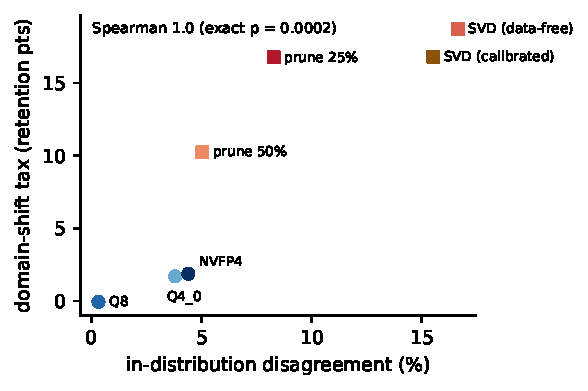
\includegraphics[width=\columnwidth]{f4_audit_scatter.pdf}
\caption{The audit. In-distribution disagreement (x-axis, forward passes only) ranks the domain-shift tax (y-axis) exactly over the seven arms. Circles: fidelity cuts. Squares: function cuts.}
\label{fig:scatter}
\end{figure}

\subsection{The statistic that failed}
\label{sec:audit-failed}

Our first audit scored the concentration of disagreements in rare-token bins, on the mechanism's logic that function cuts damage rare continuations. It failed on both families, and the numbers show how badly: the 4-bit arms' rare-share of disagreement (0.32 to 0.33) sits inside the function arms' range (0.23 to 0.38). Quantized arms also disagree disproportionately on rare tokens, harmlessly, by tie-flip, since rare-token logit margins are thin. The low-rank arms damage all bins. Rarity-concentration measures where disagreements sit; harm rate measures what they cost, and only cost separates the families. We report this because instrument design is the contribution: the obvious statistic reads plausibly and misclassifies every quantized arm.

\section{Why Selection Fails: The Tail Is Statistically Invisible}
\label{sec:mechanism}

\subsection{Rare function, rare evidence}
\label{sec:rare}

An activation statistic assigns each channel the evidence its firing history provides. A channel that serves common syntax fires at every position and dominates any ranking. A channel that serves rare content, an uncommon language, a technical register, an unusual construction, fires on the rare positions that need it. Over a finite calibration sample its accumulated mass is indistinguishable from a useless channel's. The selection problem is therefore ill-posed for exactly the parameters that carry shifted-content function: the calibration data that would reveal them is by definition the data the deployment has never seen. The two function-cut geometries delete differently under this one mechanism. Pruning removes whole channels, so its damage lands where those channels fired, in the rare-token bins; low-rank factorization removes small spectral directions, whose loss spreads over every position. Mass and spectrum are both statistics of typical data, and both go blind at the same place. Widening the sample does not help at any width we tested (12 to 100 documents, and an online mask over the live stream itself), because the tail scales with the sample.

The divergence-conditioned scheme sharpens the point. We restored pruned channels ranked by their activation at the exact positions where the pruned head fails, the most failure-targeted statistic available without gradients. It recovered less accuracy than restoring channels by plain global mass. Even conditioning on observed failures does not expose the tail, because at those positions the missing channels are missing: they cannot fire in the pruned network that produced the failures.

\subsection{Superposition blocks the shortcut}
\label{sec:superposition}

Vocabulary trim suggests a shortcut: after deleting 87\% of the output rows, some block machinery should serve only the deleted rows and die harmlessly. We measured it. For every FFN channel we computed the fraction of its output-projection energy landing on hot rows. The distribution is a narrow band (0.116 to 0.159 across all 12,288 channels) around the hot vocabulary's share of total energy (Figure~\ref{fig:hotratio}). Every channel spreads its influence across the whole vocabulary in near-uniform proportion, the signature of features stored in superposition. Trim therefore orphans no computation, which explains both of its properties at once: it is shift-proof because it removes no function, and it creates no pruning headroom because no function became dead.

\begin{figure}[t]
\centering
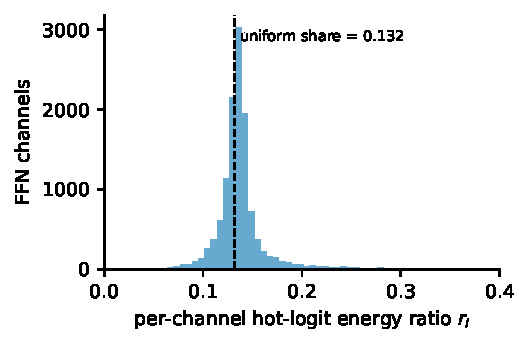
\includegraphics[width=\columnwidth]{f5_hot_ratio.pdf}
\caption{Hot-logit energy ratio for all 12,288 FFN channels. The distribution peaks at the hot vocabulary's uniform share (dashed line): no channel specializes in the trimmed vocabulary, so trim orphans nothing that pruning could harvest.}
\label{fig:hotratio}
\end{figure}

\subsection{Falsified explanations}
\label{sec:falsified}

Two mechanisms we believed earlier failed their tests, and both failures tightened the result. First, carrier compounding: we hypothesized that pruning corrupts the hidden state each draft step passes to the next, compounding down the chain. Teacher-forced chain measurements refuted it: the pruned head holds 97\% of the full head's chain acceptance on calibration-register text, in torch and in the engine. The damage is content-conditional and needs no error accumulation. Second, rarity-concentration as the audit signal (\S\ref{sec:audit-failed}): where disagreements sit does not separate the families; what they cost does. The surviving mechanism is the statistical one above, and it makes one falsifiable prediction the data confirms: the tax must grow with shift distance, because shift raises the frequency of positions whose machinery was invisible at selection time. Retention falls monotonically from held-out (97 to 99\%) through same-register (95 to 97\%) to domain shift (71 to 88\%) for every function cut, while every fidelity cut stays within two points across the whole range.

\section{Related Work}
\label{sec:related}

\textbf{Speculative decoding with cheap drafts.} FR-Spec \cite{zhao2025frspec} trims the draft vocabulary at load time and reports 1 to 3\% end-to-end gain in llama.cpp, and follow-up work casts draft vocabulary size as a coverage-versus-latency optimization for separate draft models \cite{benshoham2026trimming}. On a bandwidth-optimized engine we measure trim alone at 1.8 to 2.7\x, and it composes with quantization. QSpec \cite{zhao2024qspec} and ML-SpecQD \cite{georganas2025mlspecqd} draft with quantized variants of the target model itself: QSpec switches quantization schemes within one model, ML-SpecQD direct-casts the target to MXFP4 as a plug-and-play draft. Both established that 4-bit drafting preserves acceptance; neither compresses a co-trained head (their drafts are whole-model copies measured in gigabytes), and neither analyzes which compressions are safe. A hierarchical-framework study \cite{zhang2025specquant} evaluates speculative decoding on quantized targets and finds the combination fragile in the memory dimension. Medusa \cite{cai2024medusa}, EAGLE-family drafters \cite{li2024eagle}, and SlimSpec's low-rank drafter head \cite{plaksin2026slimspec} attach trained heads to models that ship none; the co-trained head's acceptance is the reason we compress it instead of replacing it.

\textbf{Compression damages the tail.} Hooker et al.\ established with Pruning Identified Exemplars \cite{hooker2019compressed} that pruned vision classifiers sacrifice underrepresented examples first, with quantization milder. LLM-era evaluations (LLM-KICK \cite{jaiswal2024kick} and successors) report broad capability loss from pruning that perplexity hides. This line measures example-level task accuracy on whole models with one cut type at a time. We add four things: the token-level oracle (millions of exact labels per GPU-hour), the 2$\times$2 design separating dimensionality from calibration-dependence, the six-scheme selection study that turns an observation into a selection-theoretic account, and the dose-response measurement across three shift distances. The taxonomy's practical half, the harm-rate audit, has no counterpart in this line: prior work diagnoses damage post hoc on curated test sets, where the audit predicts it pre-deployment from in-distribution forward passes.

\textbf{Quantization robustness.} The QAT and post-training-quantization literature long ago established that uniform quantization degrades gracefully; we claim no priority there. Our contribution is comparative and mechanistic: at matched in-distribution retention, quantization's damage stays flat under distribution shift while every selective cut's damage grows, and the difference traces to what each cut removes.

\section{Playbook and Limitations}
\label{sec:playbook}

\subsection{Constraint to cut}
\label{sec:constraint}

Table~\ref{tab:playbook} maps deployment constraints to the safe cut.

\begin{table*}[t]
\caption{The playbook: deployment constraint to safe action.}
\label{tab:playbook}
\vskip 0.1in
\centering
\small
\begin{tabular}{p{4.6cm}p{5.4cm}p{5.4cm}}
\toprule
Your situation & Do this & Expect \\
\midrule
Model ships a co-trained head; decode is bandwidth-bound & Trim + NVFP4 (the recipe, \S\ref{sec:recipe}) & 1.8 to 2.7\x{} over plain decode; 212 to 259MB artifact; no training \\
\addlinespace
Memory pressure demands more than 4-bit trim delivers & Stop. Pruning and low-rank buy at most 90MB more and pay 10 to 19 acceptance points on shifted traffic & Run the audit (\S\ref{sec:audit}) before believing any further cut \\
\addlinespace
Compressed draft from any source, provenance unknown & Audit it: harm rate under 0.15 is noise-type, above 0.25 is function-type & Minutes of forward passes; Spearman 1.0 tax ranking on our hardest suite \\
\addlinespace
No co-trained head exists, or a quantized base broke it & Distill a replacement on the model's own serving-regime output (chain KD, then brief CE) & 91 to 98\% of a co-trained teacher's chain acceptance; function-cut robustness profile \\
\addlinespace
Benchmarking any sampled-decoding change & Aggregate suites with 3+ seeds; never single prompts & Single-prompt sampled cells swing 12 points across seeds \\
\bottomrule
\end{tabular}
\end{table*}

\subsection{Limitations}
\label{sec:limitations}

The evidence covers one model family (Qwen3.5-9B, Qwen3.6-27B) and one engine, with an independent third configuration reproducing the recipe's pattern. Speedup magnitudes are engine-specific; acceptance and retention are not, since teacher-forced torch measurements and live engine chains agree (\S\ref{sec:falsified}). Other architectures' heads may sit differently on the cost curve. The taxonomy's mechanism (\S\ref{sec:mechanism}) has no model-specific ingredient. The impossibility result covers zero-training, statistics-based selection; gradient-informed selection and prune-then-finetune recovery sit outside the zero-training envelope this paper commits to, and could in principle re-earn their cuts. The audit requires the uncompressed reference head for its comparison passes. The domain-shift suite, though genuinely shifted (the reference's own accuracy drops 2.4\x), is 24 documents; the taxes it measures carry the confidence intervals of \S\ref{sec:robust}, and wider suites would tighten them. Hot-vocabulary coverage caps trim at 95 to 99\% on the registers we serve, and coverage is register-bound where retention is not: on our domain-shift suite the hot set covers 93 to 95\% of English scientific and web text but 62\% of German, 21\% of Russian, 9\% of Hebrew, and 5\% of Chinese Wikipedia tokens, while the 4-bit arms keep at least 97.5\% within-hot retention on those same corpora. A deployment serving registers outside its hot set needs its vocabulary re-ranked, and the check is cheap: coverage is a token count on any traffic sample, and re-export takes minutes.

\bibliography{references}
\bibliographystyle{mlsys2025}

\appendix

\section{The Six Selection Schemes}
\label{app:schemes}

Table~\ref{tab:schemes} gives the per-scheme cells behind \S\ref{sec:selection}. Every scheme either reproduces the global-mass baseline or loses to it; none removes the function-cut tax.

\begin{table}[h]
\caption{Six zero-training selection schemes for channel pruning, with each scheme's decisive measurement. Retention values are teacher-forced accuracy relative to the reference head unless noted.}
\label{tab:schemes}
\vskip 0.1in
\centering
\small
\begin{tabular}{p{2.5cm}p{4.7cm}}
\toprule
Scheme & Decisive cell \\
\midrule
Global activation mass (baseline) & In-dist retention 97.2\%; domain-shift retention 80.4\% (the tax every other scheme tries to remove) \\
\addlinespace
Wanda-style act$\times$$\|$w$\|$ & Ranking overlap with mass 88\%; chain acceptance 0.712 vs.\ mass 0.712; identical live acceptance \\
\addlinespace
Wide calibration (100 docs, max-over-docs) & Rankings identical to 12-doc mass; live acceptance 41.7\% vs.\ 41.3\% \\
\addlinespace
Online EMA mask (updated on the served stream) & 0.846 vs.\ 0.844 for the static mask; mask calibrated on the stream itself matches the corpus mask (0.854 both) \\
\addlinespace
Vocabulary-conditioned (hot-logit energy) & Worse than mass: 93.8\% vs.\ 97.1\% in-dist retention; the energy ratio is uniform across all channels (Figure~\ref{fig:hotratio}) \\
\addlinespace
Divergence-conditioned (restore by activation at observed failure positions) & Recovers less than restoring by global mass: 0.854/0.805 vs.\ 0.860/0.807 (in-dist/shift accuracy); restored sets overlap 102 of 614 channels \\
\bottomrule
\end{tabular}
\end{table}

\section{Leave-One-Domain-Out Ranking Stability}
\label{app:lodo}

The audit's Spearman 1.0 ranking (\S\ref{sec:audit-validation}) could in principle depend on one domain of the shift suite. It does not. Re-running the audit per domain (800 positions each) and recomputing the disagreement-to-tax correlation with each domain removed keeps the Spearman between 0.964 and 1.000 for all six drops (the 0.964 cases are one adjacent-pair swap among the function cuts). The family gap survives every drop: fidelity taxes stay at or under 2.5 points and function taxes at or above 5.0 points in the worst case (dropping German Wikipedia, the largest-coverage-loss domain).

\end{document}
